\subsection{Dns Script}
\begin{figure}[htp]
\centering
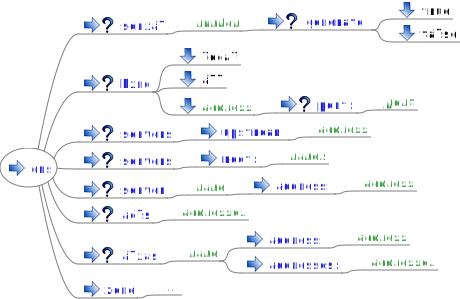
\includegraphics[angle=90,height=0.7\textheight]{dns_service_script}
\label{fig:dns_script_statements}
\caption{Dns Script Statements}
\end{figure}


\TheStatement{dns}
\TheStatement*[dns]{dns \{ serial bind servers server acls alias zone \}}

Entry point in the dns script.

% serial
\TheStatement[dns:serial]{serial}
\TheStatement*[dns!serial]{serial \Arg{number} [, generate: true|false]}

Sets the serial \Arg{number} of the zone records.
The serial number can be any number, it is added to the automatically
generated serial. The DNS service needs the serial number to be updated
for all records that have been changed. The service can create serial
numbers based on the current date but the user needs to update this
serial number if the records are changed more then once in a day.
If generate is set to \code{true} then the serial number is added to
the automatically generated serial, otherwise the serial number is used 
as specified.

\begin{lstlisting}[style=Java]
dns {
    serial 99, generate: false
}
\end{lstlisting}

% bind
\TheStatement[dns:bind]{bind}
\TheStatement*[dns!bind]{bind [local|all|\Arg{address} [, port: \Arg{port}]}

The IP \Arg{address} or a list of addresses or the host name(s) 
on which the dns server should listen to connections. Set to \qcode{local}
for the local host address \code{127.0.0.1} or to \qcode{all} to listen to all
hosts. Optionally, the \Arg{port} the dns server should listen.

\begin{lstlisting}[style=Java]
dns {
    bind local, port: 53
}
\end{lstlisting}

% servers upstream
\TheStatement[dns:servers:upstream]{servers}
\TheStatement*[dns!servers!upstream]{servers upstream: \Arg{server}}

Sets the upstream \Arg{server} or servers. Can be used multiple times
for different servers.

\begin{lstlisting}[style=Java]
dns {
    servers upstream: "8.8.8.8"
}
\end{lstlisting}

% servers root
\TheStatement[dns:servers:root]{servers}
\TheStatement*[dns!servers!root]{servers root: \Arg{server}}

Sets the root \Arg{server} or servers. Can be used multiple times
for different servers.

\begin{lstlisting}[style=Java]
dns {
    servers root: "icann"
}
\end{lstlisting}

% server
\TheStatement[dns:server]{server}
\TheStatement*[dns!server]{server \Arg{name}, address: \Arg{address}}

Sets the named root \Arg{server} and its \Arg{address}. Can be used multiple times
for different server.

\begin{lstlisting}[style=Java]
dns {
    server "example1.com", address: "127.0.0.2"
    server "example2.com", address: "127.0.0.3"
}
\end{lstlisting}

% alias
\TheStatement[dns:alias]{alias}
\TheStatement*[dns!alias]{alias \Arg{name}, address: \Arg{address}}

Sets the \Arg{alias} and its \Arg{address}. Can be used multiple times
for different aliases.

\begin{lstlisting}[style=Java]
dns {
    alias "localhost", address: "127.0.0.1"
    alias "vbox", addresses: "10.0.2.2, 10.0.2.3"
}
\end{lstlisting}

% acls
\TheStatement[dns:acls]{acls}
\TheStatement*[dns!acls]{acls \Arg{address}}

Sets the ACLs \Arg{address} or addresses. Can be used multiple times
for different aclses.

\begin{lstlisting}[style=Java]
dns {
    acls "127.0.0.1"
    acls "192.168.0.1, 192.168.0.2"
}
\end{lstlisting}

% zone
\TheStatement[dns:zone]{zone}
\TheStatement*[dns!zone]{\mbox{zone \Arg{name},} \mbox{primary: \Arg{primary},} \mbox{email: \Arg{email} [,} \mbox{serial: \Arg{serial}]\} [,} \mbox{address: \Arg{address}] [,} \mbox{ttl: \Arg{time}] [,} \{ [ttl] [refresh] [retry] [expire] \\\mbox{record \} ]}}

Adds a new DNS zone. The \Arg{name}, the \Arg{primary} DNS server and 
the \Arg{email} address of the zone are required. The \Arg{serial} number can
be set for the DNS zone.
An A-record for the zone
can be created if the IP \Arg{address} of the zone is specified. If the
TTL \Arg{time} is specified it is set for the A-record.

\begin{lstlisting}[style=Java]
dns {
    zone "example1.com", primary: "ns.example1.com", email: "hostmaster@example1.com", {
    }
}
\end{lstlisting}

\TheStatement[dns:ttl]{ttl}
\TheStatement*[dns!ttl]{ttl duration: \Arg{duration} [, minimum: \Arg{duration}]}

Sets the time to live \Arg{duration}. 
The duration accepts ISO 8601 time formats.

\TheStatement[dns:refresh]{refresh}
\TheStatement*[dns!refresh]{refresh duration: \Arg{duration}}

Sets the refresh time \Arg{duration}.
The duration accept ISO 8601 time formats.

\TheStatement[dns:retry]{retry}
\TheStatement*[dns!retry]{retry duration: \Arg{duration}}

Sets the retry time \Arg{duration}.
The duration accept ISO 8601 time formats.

\TheStatement[dns:expire]{expire}
\TheStatement*[dns!expire]{expire duration: \Arg{duration}}

Sets the expire time \Arg{duration}.
The duration accept ISO 8601 time formats.

\begin{lstlisting}[style=Java]
dns {
    zone "example1.com", primary: "ns.example1.com", email: "hostmaster@example1.com", {
        ttl duration: "PT5S"
        refresh duration: "PT20S"
        retry duration: "PT20S"
        expire duration: "PT20S"
        minimum_ttl duration: "PT20S"
    }
}
\end{lstlisting}

\TheStatement[dns:record]{record}
\TheStatement*[dns!record]{record a|ns|mx|cname [, name: \Arg{name}] [, alias: \Arg{alias}] \} [,\\ \mbox{address: \Arg{address}] [,} priority: \Arg{priority}] [, \{ ttl \}]}

Adds a new DNS record to the DNS zone. 
The accepted arguments are depending on
the record type. The \qcode{a} record type will add a new A-record with the 
specified \Arg{name} and \Arg{address}; 
the \qcode{ns} record type will add a 
new NS-record with the specified \Arg{name}. If 
the \Arg{address} of the NS-record is specified then a new A-record will be 
created that maps this name to the specified address and uses the 
same TTL duration;
the \qcode{mx} record type will add a 
new MX-record with the specified \Arg{name}. 

Optionally, the \Arg{priority}
of the MX-record can be set. If the \Arg{address} of the MX-record is 
specified then a new A-record will be created that maps this name to the 
specified address and uses the same TTL duration;
the \qcode{cname} record type will add
a new CNAME-record with the specified \Arg{name} and \Arg{alias}.
The placeholder \qcode{\%} can be used that is replaced by the current zone.

\begin{lstlisting}[style=Java]
dns {
    zone "example1.com", primary: "ns.example1.com", email: "hostmaster@example1.com", {
        record a, name: "testa.com", address: "192.168.0.51"
        record a, name: "testb.com", address: "192.168.0.52", { 
            ttl duration: "PT24H" 
        }
        record ns, name: "ns1.testa.com"
        record mx, name: "mx2.testa.com", priority: 20
        record cname, name: "www.testa.com", alias: "testa.com"
    }
}
\end{lstlisting}

